%Goals
% You can use std::array and std::vector in your code
% You can use an iterator to access container elements
% You can access and modify container contents using algorithms
% You can interact with streams through iterators

\section{Iterators}
There are always two iterators used (begin() und end()). There is also the possibility to traverse a list from front to back (rbegin() and rend()). If the members are only read the const version (cbegin() and cend()) can be used.

\subsection{Iteration}
Its possible to index a vector like an array but there is no bounds check.    Accessing an element outside the valid range is Undefined Behavior.

\textbf{Bad Style Iteration!}\\
\begin{lstlisting}[language=C++]
for (size_t i = 0; i < v.size(); ++i) {  //Index is "unsigned" 0-1=MAX_INT
	std::cout << "v[" << i << "] = " << v[i] << '\n'; }
}	
\end{lstlisting}

\textbf{Element Iteration (Range-Based for)}
\begin{itemize}
  \itemsep -0.5em 
  \item Advantage: No index error possible 
  \item Works with all containers, even value lists {1, 2, 3}
\end{itemize}

\begin{center}
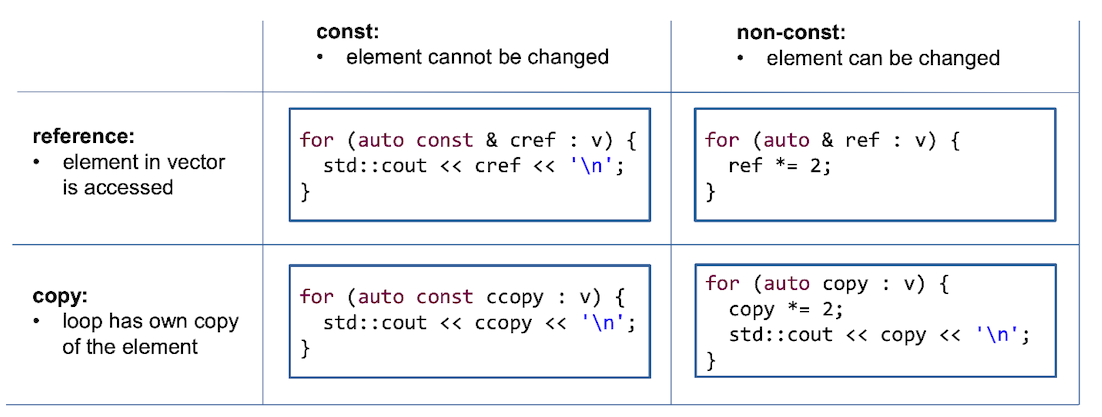
\includegraphics[width=0.75\linewidth]{images/elementiteration}	
\end{center}

\textbf{Iteration with Iterators}
\begin{lstlisting}[language=C++]
for (auto it = std::begin(v); it != std::end(v); ++it) {
	std::cout << (*it)++ << ", "; 
}
// Guarantee to just have read-only access with std::cbegin() and std::cend()
for (auto it = std::cbegin(v); it != std::cend(v); ++it) {
	std::cout << *it << ", "; 
}
\end{lstlisting}

\subsection{Using Iterators with Algorithms}
 Each algorithm takes iterator arguments. The algorithm does what its name tells us. 
 
\begin{lstlisting}[language=C++]
// Counting blanks in a string
size_t count_blanks(std::string s) {
 	size_t count{0};
 	for (size_t = 0; i < s.size(); ++i) {
 		if (s[i] == ' ') {
 			++count;
 		}
 	}
 	return count;
 }
 
// Counting blanks in a string with algorithms
size_t count_blanks(std::string s) {
	return std::count(s.begin(), s.end(), ' ');
}

// Summing up all values in a vector
std::vector<int> v{5, 4, 3, 2, 1}; 
std::cout << std::accumulate(std::begin(v), std::end(v), 0)<< " = sum\n";

// Number of elements in range 
void printDistanceAndLength(std::string s) {
	std::cout << "distance: "<< std::distance(s.begin(), s.end()) <<'\n';
	std::cout << "in a string of length: "<< s.size()<<'\n'; 
} 	

// Printing all values of a vector
void printAll(std::vector<int> v) {
	std::for_each(std::crbegin(v), std::crend(v), print); 
}

// For each with a Lambda
void printAll(std::vector<int> v, std::ostream & out) {
	std::for_each(std::crbegin(v), std::crend(v), [&out](auto x) {
		out << "print: "<< x << '\n';
	});
}

\end{lstlisting}


\subsection{Iterators for I/O}
Iterators connect streams and algorithms.  Streams (std::istream and std::ostream) cannot be used with algorithms directly.
\begin{itemize}
	\itemsep -0.5em 
  	\item \lstinline{std::ostream_iterator<T>} outputs values of type T to the given std::ostream
  	\begin{itemize}
  		\item No end() marker needed for output, it ends when the input range ends.
  	\end{itemize}
  	
  	\item  \lstlinline|std::istream_iterator<T>| reads values of type T from the given std::istream
	\begin{itemize}
  		\item End iterator is the default constructed \lstinline|std::istream_iterator<T>{}|
   		\item It ends when the stream is no longer good().
   	\end{itemize}
\end{itemize}

\subsection{Types}
There are five different types of iterators in C++.
\begin{lstlisting}[language=C++]
struct input_iterator_tag { };
struct output_iterator_tag { };
struct forward_iterator_tag : public inputer_iterator_tag { };
struct bidirectional_iterator_tag : public forward_iterator_tag { };
struct random_access_iterator_tag : public bidirectional_iterator_tag { };
\end{lstlisting}

\subsubsection{Input Iterator}
\begin{itemize}
  \itemsep -0.5em 
  \item The element can be read only once and after that the iterator has to be incremeneted.
  \item Used for \lstinline[language=C++]|std::istream_iterator| and \lstinline[language=C++]|std::istreambuf_iterator|
\end{itemize}

\subsubsection{Forward Iterator}
\begin{itemize}
  \itemsep -0.5em 
  \item Element can be read in and changed (Except element or container is const).
  \item Only allows forward iteration
  \item Sequenz can be iterated over multiple times
\end{itemize}

\subsubsection{Bidirectional Iterator}
\begin{itemize}
  \itemsep -0.5em 
  \item Element can be read in and changed (Except element or container is const).
  \item Allows forward and backwards iteration
  \item Sequenz can be iterated over multiple times
  \item The random access iterator behaves as the bidirectional iterator with the addition that the can access elements over the index
\end{itemize}

\subsubsection{Output Iterator}
\begin{itemize}
  \itemsep -0.5em 
  \item Current element can be changed once, after that the iterator has to be incremented.
  \item There is no end for this iterator (example console prints)
  \item Used for \lstinline|std::ostream_iterator|
  \item Writes the result without knowing the result.
\end{itemize}




\break